\documentclass[tikz,border=8pt]{standalone}
\usepackage{tikz}
\usepackage{tkz-euclide}
\usepackage{amsmath, amssymb}

\usetikzlibrary{angles, quotes}

\begin{document}

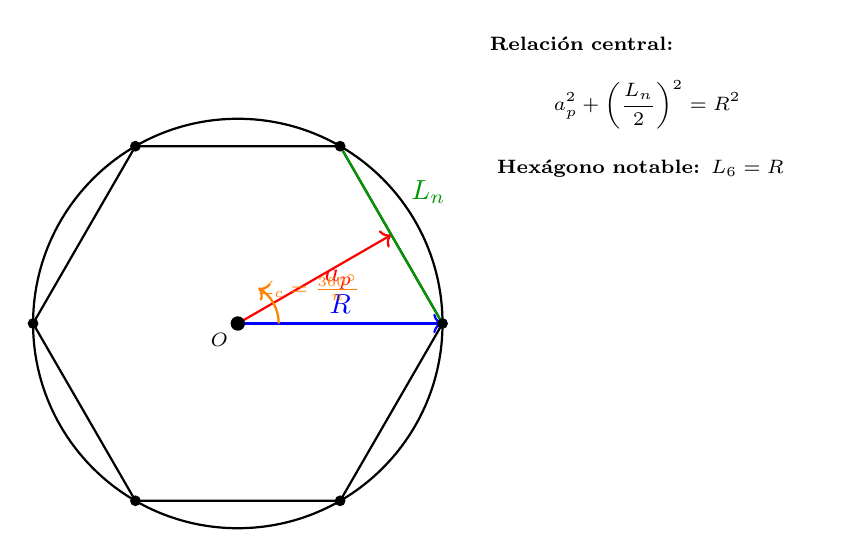
\begin{tikzpicture}[scale=1.3]

  % ---- Hexágono regular inscrito en círculo ----
  \coordinate (O) at (0,0);
  \draw[thick] (O) circle (2);
  \draw[thick] (0:2) -- (60:2) -- (120:2) -- (180:2) -- (240:2) -- (300:2) -- cycle;

  % ---- Radio R y apotema a_p ----
  \draw[blue, thick, ->] (O) -- (0:2) node[midway, above] {$R$};
  \draw[red, thick, ->] (O) -- (30:1.732) node[midway, right] {$a_p$};
  \draw[red, dashed] (30:1.732) -- (60:2);
  \draw[red, dashed] (30:1.732) -- (0:2);

  % ---- Lado L_n ----
  \draw[green!60!black, thick] (0:2) -- (60:2);
  \node[green!60!black, above] at (30:2.15) {$L_n$};

  % ---- Ángulo central ----
  \draw[->, orange, thick] (0.4,0) arc (0:60:0.4);
  \node[orange] at (0.7,0.35) {\scriptsize $\angle_c = \frac{360^\circ}{n}$};

  % ---- Centro y vértices ----
  \fill (O) circle (2pt) node[below left] {\scriptsize $O$};
  \foreach \ang in {0,60,120,180,240,300} {
    \fill (\ang:2) circle (1.5pt);
  }

  % ---- Cuadrante rectángulo para mostrar relación a_p, L_n/2, R ----
  \node[align=left, text width=4cm, font=\scriptsize] at (4, 2) {
    \textbf{Relación central:}
    $$a_p^2 + \left(\frac{L_n}{2}\right)^2 = R^2$$
    \vspace{0.3cm}
    \textbf{Hexágono notable:} $L_6 = R$
  };

\end{tikzpicture}

\end{document}
